

\documentclass[landscape,final,a0paper,fontscale=0.285]{baposter}
    \renewcommand{\refname}{}
\usepackage{calc}
\usepackage{graphicx}
\usepackage{epstopdf}
\usepackage{amsmath}
\usepackage{amssymb}
\usepackage{relsize}
\usepackage{multirow}
\usepackage{rotating}
\usepackage{bm}
\usepackage{url}
\usepackage{cite}
\usepackage{graphicx}
\usepackage{multicol}

%\usepackage{times}
%\usepackage{helvet}
%\usepackage{bookman}
\usepackage{palatino}



\newcommand{\captionfont}{\footnotesize}

\graphicspath{{images/}{../images/}}
\usetikzlibrary{calc}

\newcommand{\SET}[1]  {\ensuremath{\mathcal{#1}}}
\newcommand{\MAT}[1]  {\ensuremath{\boldsymbol{#1}}}
\newcommand{\VEC}[1]  {\ensuremath{\boldsymbol{#1}}}
\newcommand{\Video}{\SET{V}}
\newcommand{\video}{\VEC{f}}
\newcommand{\track}{x}
\newcommand{\Track}{\SET T}
\newcommand{\LMs}{\SET L}
\newcommand{\lm}{l}
\newcommand{\PosE}{\SET P}
\newcommand{\posE}{\VEC p}
\newcommand{\negE}{\VEC n}
\newcommand{\NegE}{\SET N}
\newcommand{\Occluded}{\SET O}
\newcommand{\occluded}{o}


%%%%%%%%%%%%%%%%%%%%%%%%%%%%%%%%%%%%%%%%%%%%%%%%%%%%%%%%%%%%%%%%%%%%%%%%%%%%%%%%
%%%% Some math symbols used in the text
%%%%%%%%%%%%%%%%%%%%%%%%%%%%%%%%%%%%%%%%%%%%%%%%%%%%%%%%%%%%%%%%%%%%%%%%%%%%%%%%

%%%%%%%%%%%%%%%%%%%%%%%%%%%%%%%%%%%%%%%%%%%%%%%%%%%%%%%%%%%%%%%%%%%%%%%%%%%%%%%%
% Multicol Settings/
%%%%%%%%%%%%%%%%%%%%%%%%%%%%%%%%%%%%%%%%%%%%%%%%%%%%%%%%%%%%%%%%%%%%%%%%%%%%%%%%
\setlength{\columnsep}{1.5em}
\setlength{\columnseprule}{0mm}

%%%%%%%%%%%%%%%%%%%%%%%%%%%%%%%%%%%%%%%%%%%%%%%%%%%%%%%%%%%%%%%%%%%%%%%%%%%%%%%%
% Save space in lists. Use this after the opening of the list
%%%%%%%%%%%%%%%%%%%%%%%%%%%%%%%%%%%%%%%%%%%%%%%%%%%%%%%%%%%%%%%%%%%%%%%%%%%%%%%%
\newcommand{\compresslist}{%
\setlength{\itemsep}{1pt}%
\setlength{\parskip}{0pt}%
\setlength{\parsep}{0pt}%
}

%%%%%%%%%%%%%%%%%%%%%%%%%%%%%%%%%%%%%%%%%%%%%%%%%%%%%%%%%%%%%%%%%%%%%%%%%%%%%%
%%% Begin of Document
%%%%%%%%%%%%%%%%%%%%%%%%%%%%%%%%%%%%%%%%%%%%%%%%%%%%%%%%%%%%%%%%%%%%%%%%%%%%%%

\begin{document}

%%%%%%%%%%%%%%%%%%%%%%%%%%%%%%%%%%%%%%%%%%%%%%%%%%%%%%%%%%%%%%%%%%%%%%%%%%%%%%
%%% Here starts the poster
%%%---------------------------------------------------------------------------
%%% Format it to your taste with the options
%%%%%%%%%%%%%%%%%%%%%%%%%%%%%%%%%%%%%%%%%%%%%%%%%%%%%%%%%%%%%%%%%%%%%%%%%%%%%%
% Define some colors

%\definecolor{lightblue}{cmyk}{0.83,0.24,0,0.12}
\definecolor{lightblue}{rgb}{0.145,0.6666,1}

% Draw a video
\newlength{\FSZ}
\newcommand{\drawvideo}[3]{% [0 0.25 0.5 0.75 1 1.25 1.5]
   \noindent\pgfmathsetlength{\FSZ}{\linewidth/#2}
   \begin{tikzpicture}[outer sep=0pt,inner sep=0pt,x=\FSZ,y=\FSZ]
   \draw[color=lightblue!50!black] (0,0) node[outer sep=0pt,inner sep=0pt,text width=\linewidth,minimum height=0] (video) {\noindent#3};
   \path [fill=lightblue!50!black,line width=0pt] 
     (video.north west) rectangle ([yshift=\FSZ] video.north east) 
    \foreach \x in {1,2,...,#2} {
      {[rounded corners=0.6] ($(video.north west)+(-0.7,0.8)+(\x,0)$) rectangle +(0.4,-0.6)}
    }
;
   \path [fill=lightblue!50!black,line width=0pt] 
     ([yshift=-1\FSZ] video.south west) rectangle (video.south east) 
    \foreach \x in {1,2,...,#2} {
      {[rounded corners=0.6] ($(video.south west)+(-0.7,-0.2)+(\x,0)$) rectangle +(0.4,-0.6)}
    }
;
   \foreach \x in {1,...,#1} {
     \draw[color=lightblue!50!black] ([xshift=\x\linewidth/#1] video.north west) -- ([xshift=\x\linewidth/#1] video.south west);
   }
   \foreach \x in {0,#1} {
     \draw[color=lightblue!50!black] ([xshift=\x\linewidth/#1,yshift=1\FSZ] video.north west) -- ([xshift=\x\linewidth/#1,yshift=-1\FSZ] video.south west);
   }
   \end{tikzpicture}
}

\hyphenation{resolution occlusions}
%%
\begin{poster}%
  % Poster Options
  {
  % Show grid to help with alignment
  grid=false,
  % Column spacing
  colspacing=1em,
  % Color style
  bgColorOne=white,
  bgColorTwo=white,
  borderColor=lightblue,
  headerColorOne=black,
  headerColorTwo=lightblue,
  headerFontColor=white,
  boxColorOne=white,
  boxColorTwo=lightblue,
  % Format of textbox
  textborder=roundedleft,
  % Format of text header
  eyecatcher=true,
  headerborder=closed,
  headerheight=0.1\textheight,
%  textfont=\sc, An example of changing the text font
  headershape=roundedright,
  headershade=shadelr,
  headerfont=\Large\bf\textsc, %Sans Serif
  textfont={\setlength{\parindent}{1.5em}},
  boxshade=plain,
%  background=shade-tb,
  background=plain,
  linewidth=2pt
  }
  % Eye Catcher
  {
\includegraphics[height=5em]{img/lgpsealm.eps}}
  % 
  {\bf\textsc{The Online Architectural Sketching Interface for Simulations }\vspace{0.5em}}
  % Authors
  {\textsc{\{ Max Espinoza, Eric Zhang, Sensen Chen, Jeramey Tyler, and Barbara Cutler \}}}
  % University logo
  {% The makebox allows the  to flow into the logo, this is a hack because of the L shaped logo.
    
\includegraphics[height=5.0em]{img/logo_cs_design_1.png}
  }

%%%%%%%%%%%%%%%%%%%%%%%%%%%%%%%%%%%%%%%%%%%%%%%%%%%%%%%%%%%%%%%%%%%%%%%%%%%%%%
%%% Now define the boxes that make up the poster
%%%---------------------------------------------------------------------------
%%% Each box has a name and can be placed absolutely or relatively.
%%% The only inconvenience is that you can only specify a relative position 
%%% towards an already declared box. So if you have a box attached to the 
%%% bottom, one to the top and a third one which should be in between, you 
%%% have to specify the top and bottom boxes before you specify the middle 
%%% box.
%%%%%%%%%%%%%%%%%%%%%%%%%%%%%%%%%%%%%%%%%%%%%%%%%%%%%%%%%%%%%%%%%%%%%%%%%%%%%%
    %
    % A coloured circle useful as a bullet with an adjustably strong filling
    \newcommand{\colouredcircle}{%
      \tikz{\useasboundingbox (-0.2em,-0.32em) rectangle(0.2em,0.32em); \draw[draw=black,fill=lightblue,line width=0.03em] (0,0) circle(0.18em);}}

%%%%%%%%%%%%%%%%%%%%%%%%%%%%%%%%%%%%%%%%%%%%%%%%%%%%%%%%%%%%%%%%%%%%%%%%%%%%%%
  \headerbox{Motivation}{name=problem,column=0,row=0}{
%%%%%%%%%%%%%%%%%%%%%%%%%%%%%%%%%%%%%%%%%%%%%%%%%%%%%%%%%%%%%%%%%%%%%%%%%%%%%%


  %Images for this section
  {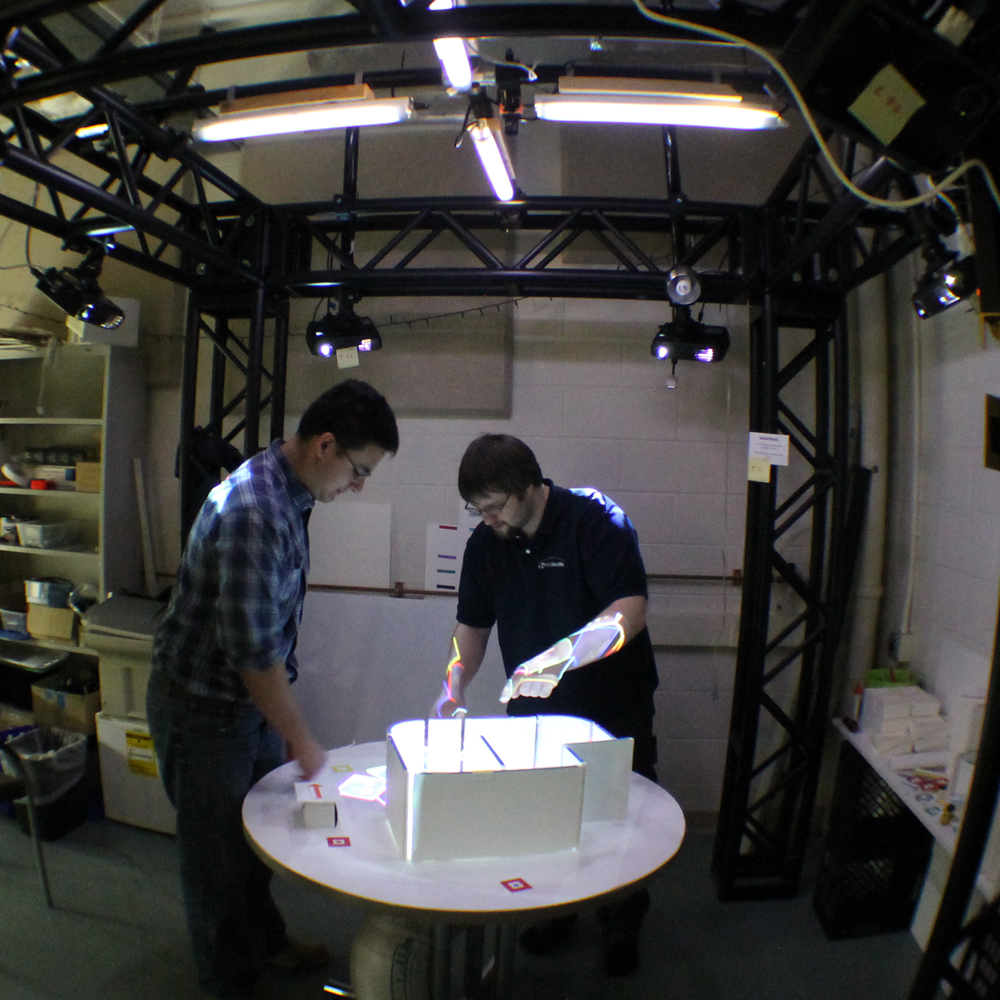
\includegraphics[height=9.5em]{img/ian_matt_contraption_frame.jpg}}
  {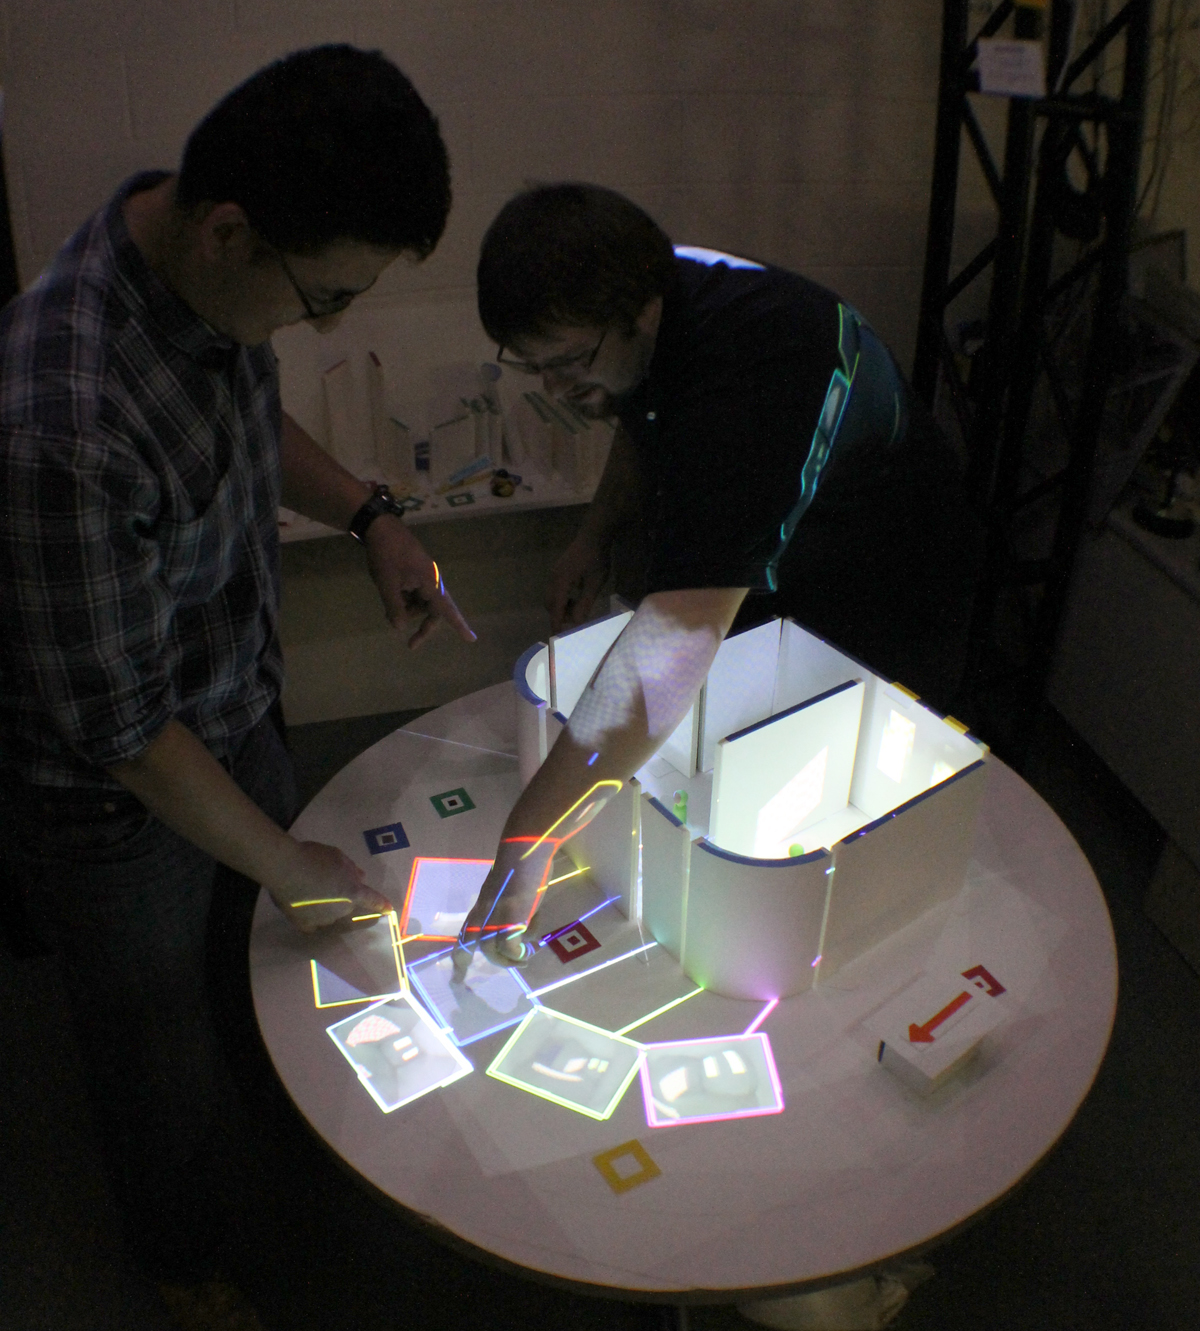
\includegraphics[height=9.5em]{img/ian_matt_pointing.jpg}}

  {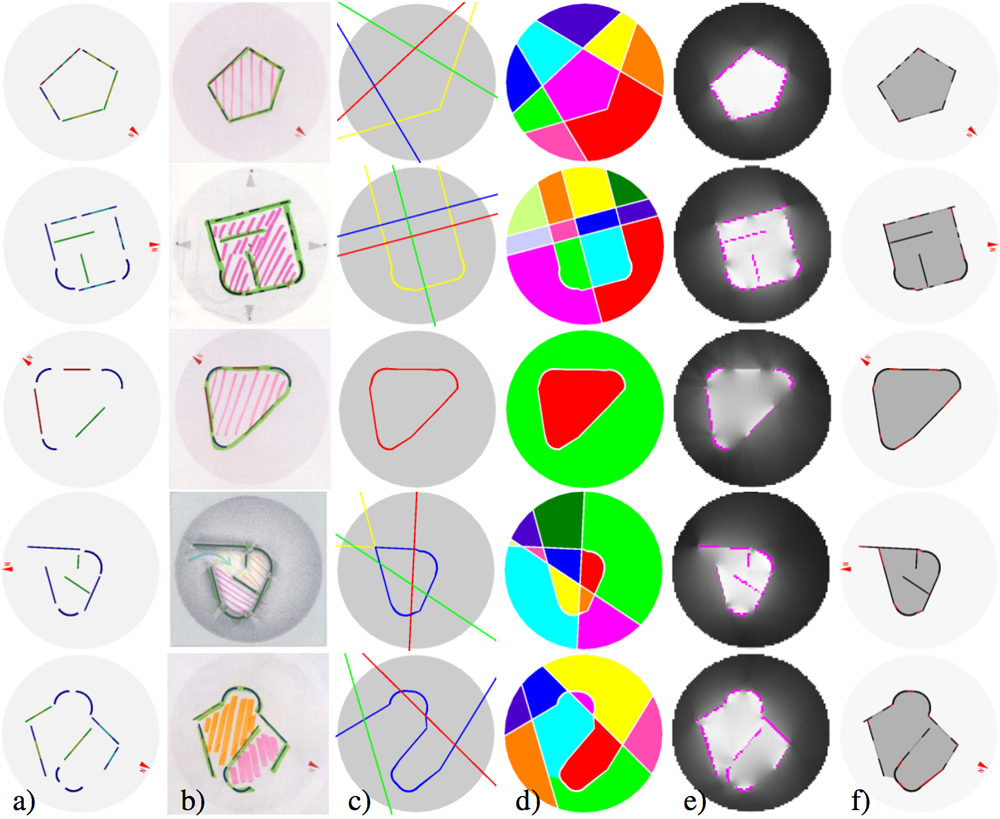
\includegraphics[height=14em]{img/aag_figure_3.png}}

  {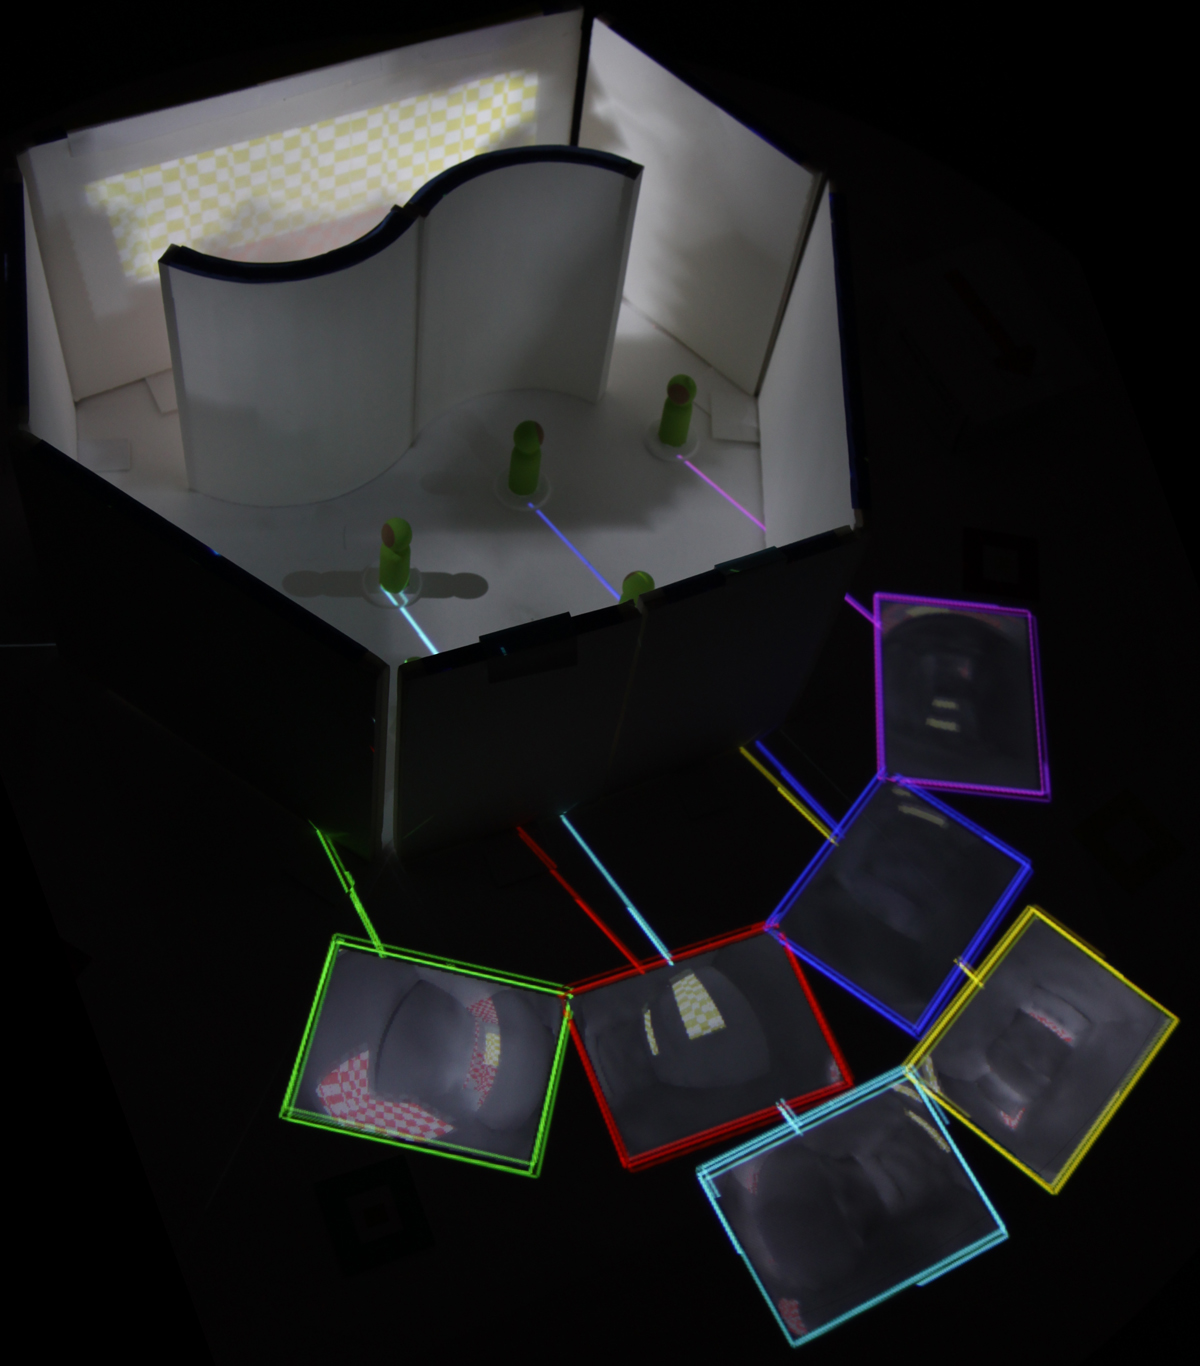
\includegraphics[height=10.5em]{img/museum_false_color2.jpg}} 
  {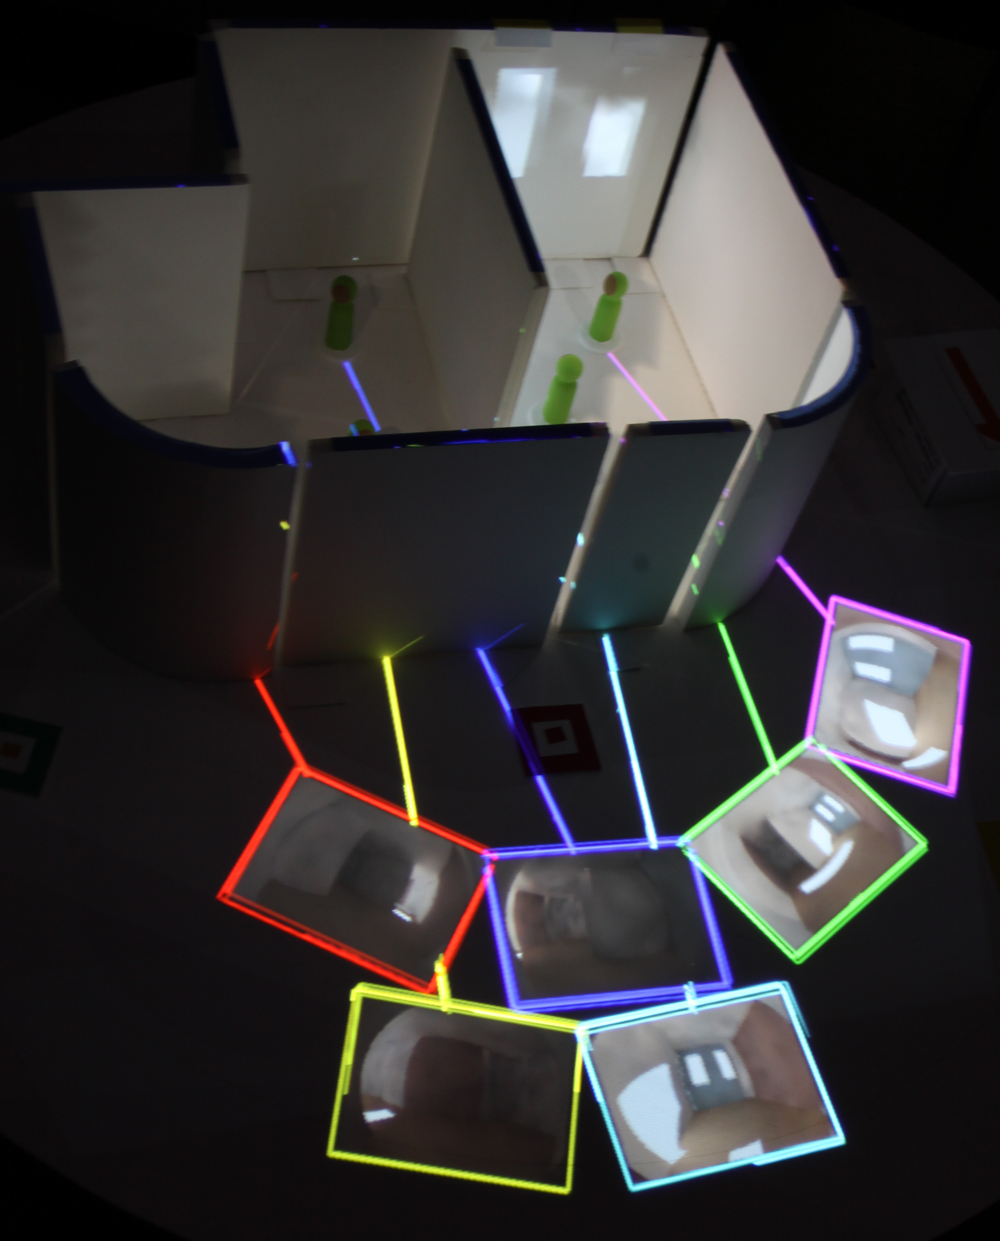
\includegraphics[height=10.5em]{img/office_color.jpg}}

  %text for this section
Previous research on the development of a spatially augmented tangible user interface for architectural daylighting simulation and design offered architects a novel approach in collaborative room design. \cite{NasmanEvaluation, ShengYYC09 }

User studies found the tools very helpful for visualizing lighting simulations and offered visual feedback to make better use of natural daylighting. Evaluation from this study lead to extending the interface to include avatars, illumination visualizations, and additional window models.\cite{NasmanEvaluation}

In order to collect more data we implemented an online interface which deliverers a set of capabilities similar to the physical system. Users are able to sketch designs which are translated into 3D models. Daylight simulated on these models relates illumination values to real world measurements.

 }%end section


%%%%%%%%%%%%%%%%%%%%%%%%%%%%%%%%%%%%%%%%%%%%%%%%%%%%%%%%%%%%%%%%%%%%%%%%%%%%%%
\headerbox{Sketching Interface}{name=userinterface,span = 2,column=2,,row=0}{
  %%%%%%%%%%%%%%%%%%%%%%%%%%%%%%%%%%%%%%%%%%%%%%%%%%%%%%%%%%%%%%%%%%%%%%%%%%%%%%
  \begin{center}{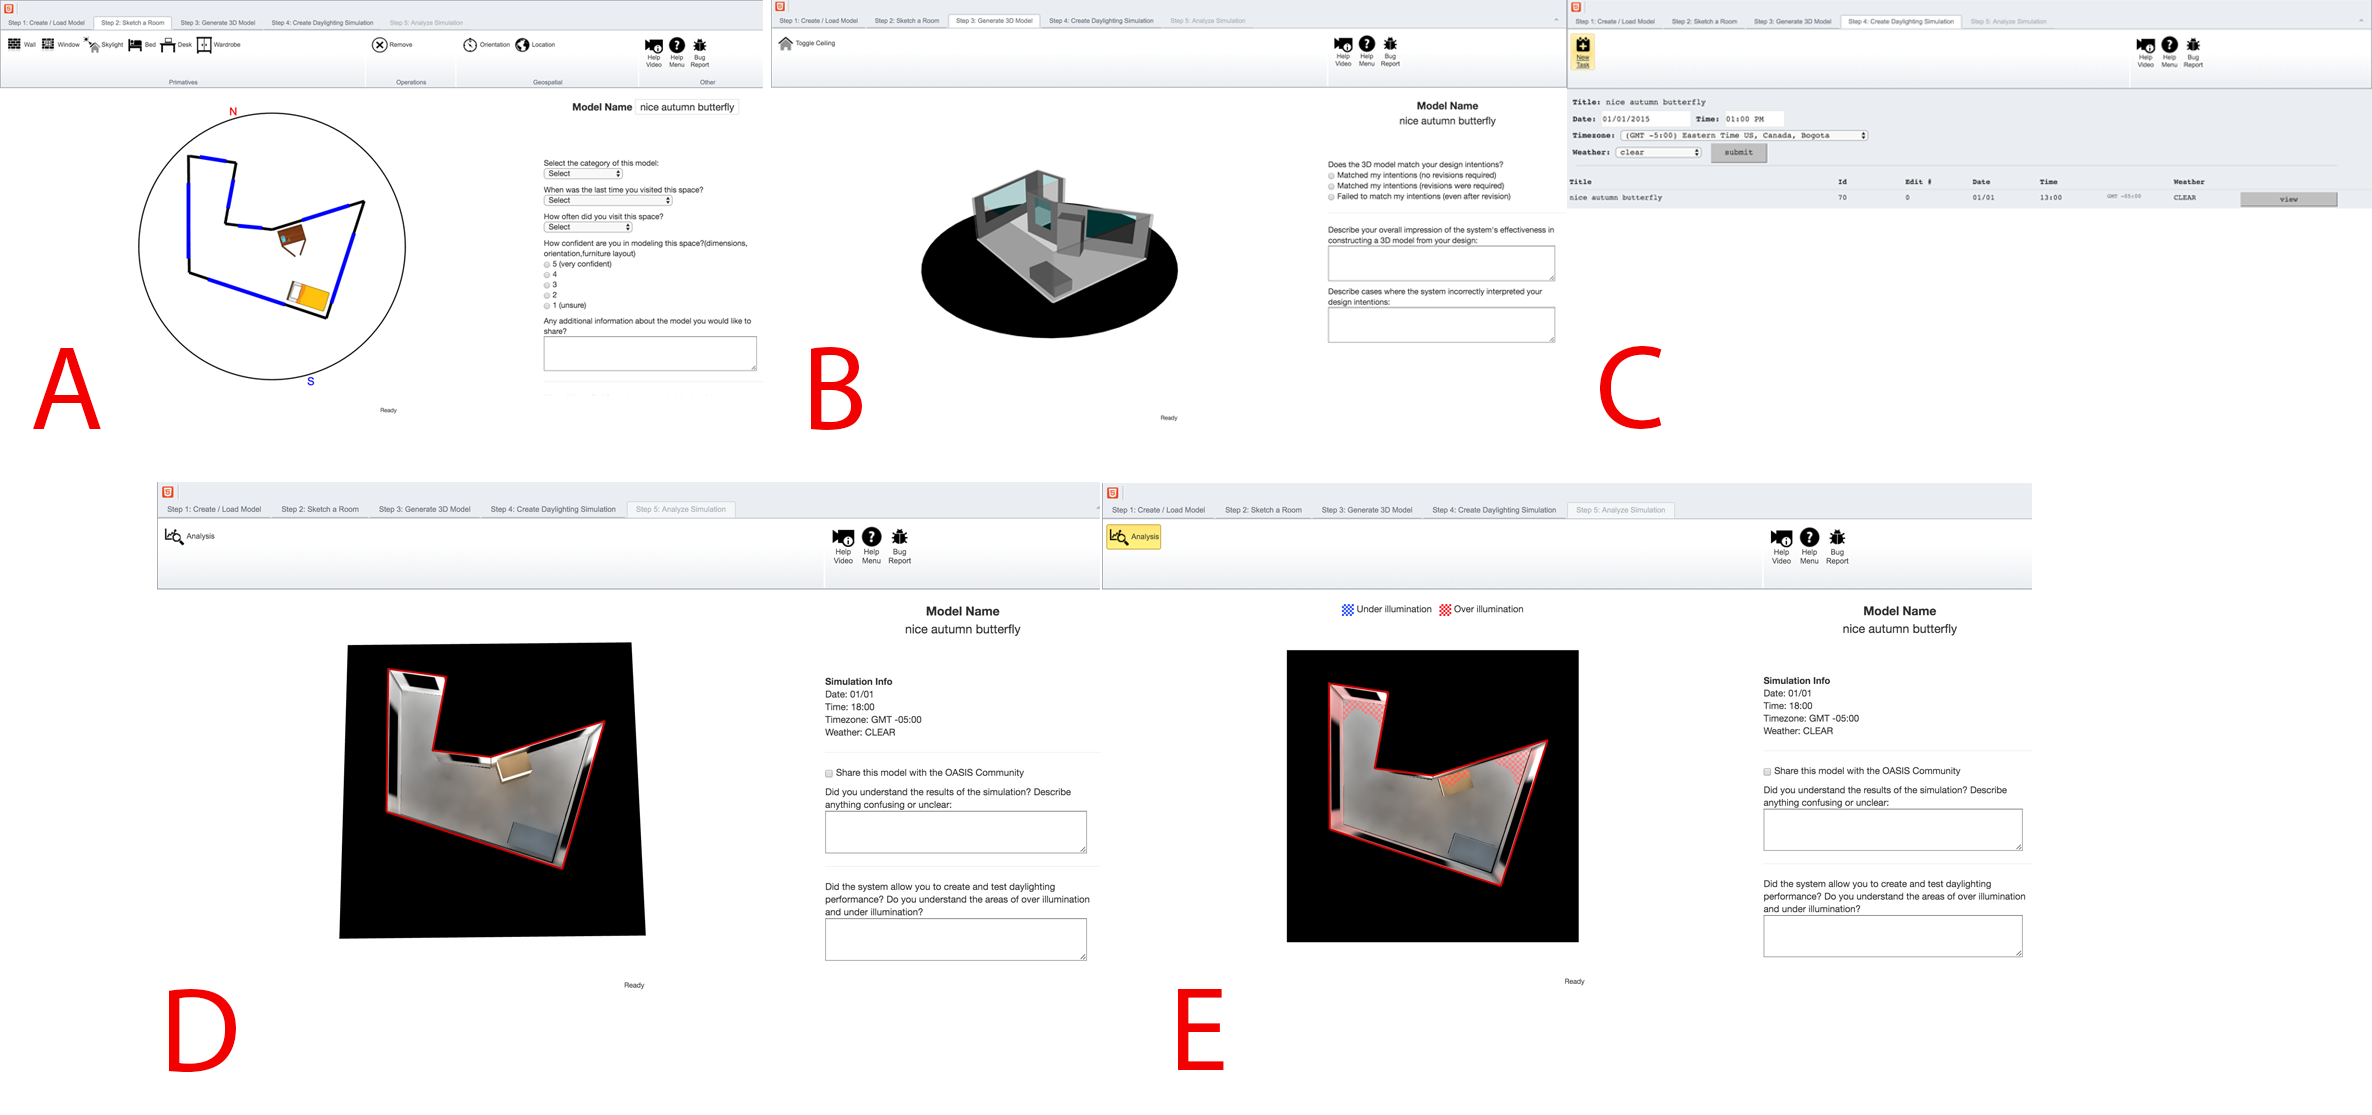
\includegraphics[width=35em]{img/pages.png}}\end{center}
  
 \begin{multicols}{2}
  	The sketching interface (A) features a variety of tools to design a space with furniture and windows. The user can change their compass orientation and geographic location. After a design is created the user can save and render the sketch by selecting the next tab on the navigation bar. The result from the rendering is a 3D geometry of the design (B). A task is a rendering of a 3D model with daylighting during a selected time.
The user can proceed to the task list (C) to create tasks or view previous tasks. Once a task is created, it will take a few seconds to be rendered. Once the task is done rendering a view button will pop up. Selecting the view button will take the user to the daylighting simulation (D). The user can view which spots are over-illuminated or under-illuminated by selecting the analyze button. The simulation analysis (E) features a room with blue spots indicating under-illumination or red spots indication over-illumination. The user can use the tool to analyze their design or change it to better utilize daylighting. \end{multicols}
  \vspace{-0.6em}
   

}

%%%%%%%%%%%%%%%%%%%%%%%%%%%%%%%%%%%%%%%%%%%%%%%%%%%%%%%%%%%%%%%%%%%%%%%%%%%%%%
  \headerbox{Contributions}{name=contribution,column=1,row=0}{
%%%%%%%%%%%%%%%%%%%%%%%%%%%%%%%%%%%%%%%%%%%%%%%%%%%%%%%%%%%%%%%%%%%%%%%%%%%%%%
  
   Currently a working prototype of the application offers functionality similar to the physical system.
   We used WebGL and the Raphael graphics libraries to build both the user interface and 3D visualization. Our online application implements the following features.
   \begin{enumerate}\compresslist
   \item A simple drag and drop interface to design models with wall primitives
   %\item Avatar primitives that render geometry to view a POV scene
   \item Save and load user created layouts
   \item Interactive feedback that allows navigation through user generated spaces with simulated daylight
   \end{enumerate}
   
\begin{center}{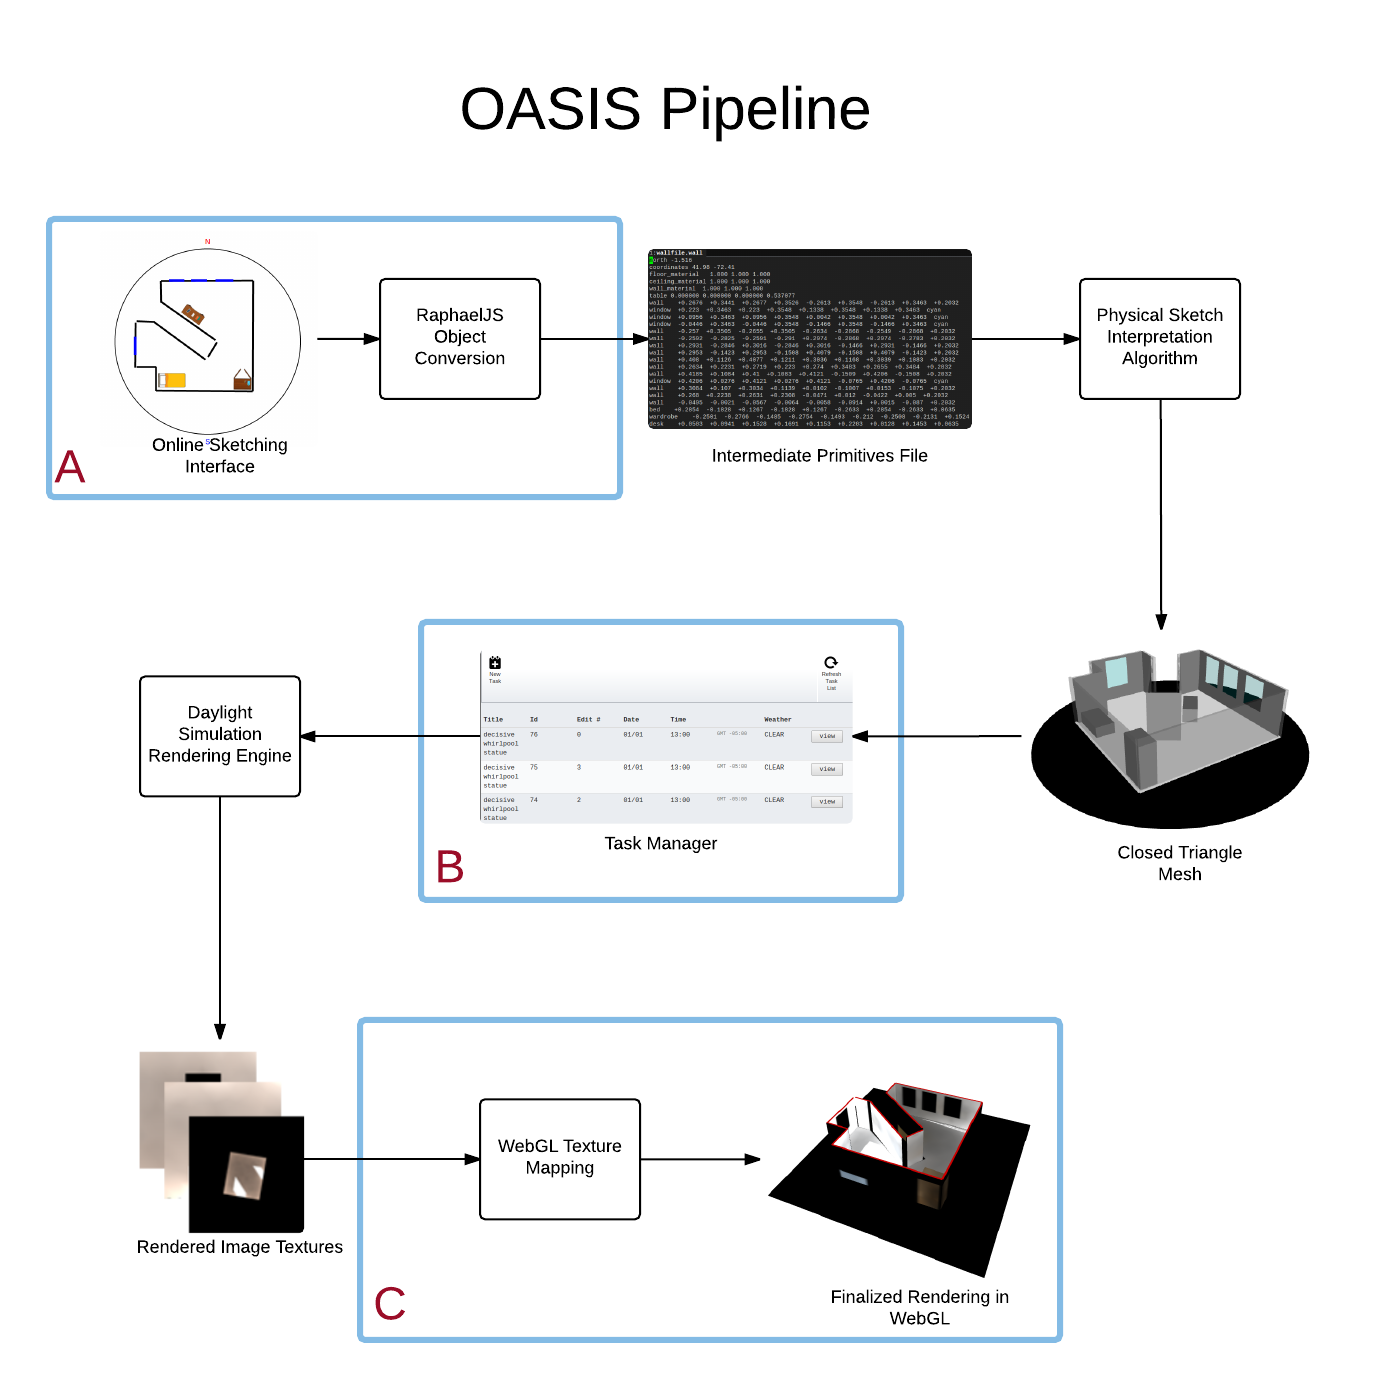
\includegraphics[width=15em]{img/new_pipeline.png}}\end{center}
The previous pipe line used a camera and image detection to create the primitive positions\cite{NasmanEvaluation, ShengYYC09 }, however with our online application we bypass image recognition and directly find the wall primitives and save those positions onto a database for later study. Those primitives go into the graphics pipeline and we get a triangle mesh model and rendered images with lighting textures, which are displayed on the screen as a 3D model. 
\vspace{1em}
    
      
   

  }

%%%%%%%%%%%%%%%%%%%%%%%%%%%%%%%%%%%%%%%%%%%%%%%%%%%%%%%%%%%%%%%%%%%%%%%%%%%%%%
\headerbox{Pilot Study}{name=future,column=2,row=1,below=userinterface,span = 2,bottomaligned=problem}{

\begin{multicols}{2}
	
	\textbf{Pilot User Study}: In addition to the creation of OASIS, we also conducted a pilot user study. 
	We hypothesize that if OASIS is publicized to users online, then anonymous online users will construct models in our sketching interface and create daylight renderings for analysis.
	Also, we speculate that the number of models anonymous online users will construct on OASIS will be quantitatively larger and from a broader range of users than previous user studies conducted on the Virtual Heliodon.
	Collecting both active and passive feedback from users will help us better understand where improvements to OASIS can be made and how users currently experience OASIS.
	Lastly, in order to collect as much feedback as possible we plan on advertising OASIS on social media outlets, online bulletin boards, and on campus.
	To summarize, we anticipate  that this pilot user study will provide us valuable feedback to improve OASIS.
	

	 
	\textbf{Share-A-Model}: The designs created with OASIS belong to the user, but we have added the option for the user to share designs with anyone. The only action the user needs to do in order to share their design is provide the unique share link associated with a model. We plan to showcase popular models that people wish to share in a gallery. 
	
	
	\begin{center}
\includegraphics[height=6em]{img/videoqr.jpg}	
	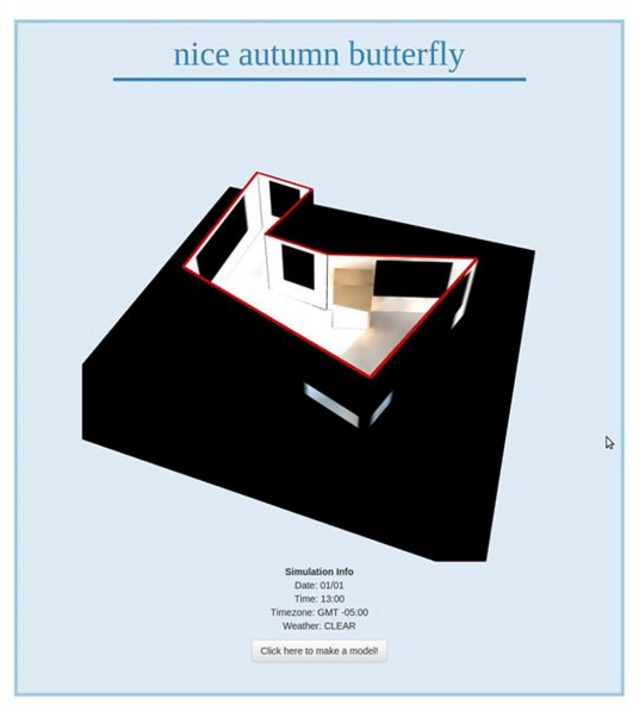
\includegraphics[height=6em]{img/nab.png}	
	\end{center}	
	
	
	
	   
 \end{multicols}
}
\headerbox{References}{name=credit, column = 1, row = 1, below = contribution, span = 1,bottomaligned=problem}{
{\tiny

\bibliography{cites}{}
\clearpage
\bibliographystyle{plain}

\par}
}

%%%%%%%%%%%%%%%%%%%%%%%%%%%%%%%%%%%%%%%%%%%%%%%%%%%%%%%%%%%%%%%%%%%%%%%%%%%%%
%%%%%%%%%%%%%%%%%%%%%%%%%%%%%%%%%%%%%%%%%%%%%%%%%%%%%%%%%%%%%%%%%%%%%%%%%%%%%%

\end{poster}
\end{document}












